% !TEX TS-program = pdflatex
% !TEX encoding = UTF-8 Unicode

% This is a simple template for a LaTeX document using the "article" class.
% See "book", "report", "letter" for other types of document.


\documentclass[a4paper,UKenglish]{lipics}
\usepackage[utf8]{inputenc} % set input encoding (not needed with XeLaTeX)
%
\usepackage{graphicx} % support the \includegraphics command and options
\usepackage{diagrams}
%
%% \usepackage[parfill]{parskip}
%
\usepackage{booktabs} 
\usepackage{array} 
\usepackage{paralist} 
\usepackage{verbatim} 
\usepackage{subfig}
\usepackage{mathtools}
\usepackage{mathpartir}
\usepackage{times}
\usepackage{amssymb}
\usepackage{float}
%\usepackage{tikz}

%\usepackage{cite}


\title{Sequential algorithms as confluent strategies between dialogue games}
\author{Clément Jacq and Paul-André Melliès}
%\institute{Laboratoire PPS, Université Paris Diderot}






\begin{document}

\maketitle

\section*{Introduction}
\hspace{1.2cm}  

\section{Dialogue Games}
\subsection{Definitions}
\begin{definition}{Dialogue Game}

A Rooted Dialogue Game is a bipartite rooted tree whose nodes are separated in two sets Cells and Values. By bipartite we mean that the children of a Value are Cells and the children of a Cell are Values. \\Additionally, a rooted dialogue game is provided with a polarising function $\lambda : Cells \oplus Values \rightarrow \{O;P\}$ such that any child of a Cell has its polarity and any child of a Value has the opposite polarity.\\
Finally, The root of a rooted dialogue game is a P-Value. \\
A Dialogue Game is a set of Rooted Dialogue Games.
\end{definition}
The basic intuition here is that we see Dialogue Games as a game semantics expansion of Berry's and Curien's Concrete Data Structures where we symetrize these structures by assigning cells and values to different players.\\ Next, we introduce the relations used to simulate the idea that a Cell can only be filled by one Value at a time in a play of the game.

\begin{figure}\centering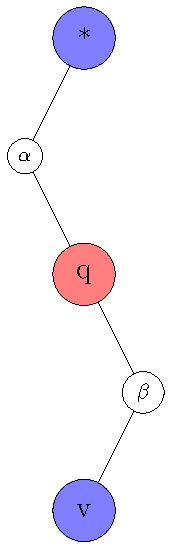
\includegraphics[scale=0.6]{dialoguegame1.pdf}\caption{An Example of Rooted Dialogue Game of root *} \end{figure}

\begin{definition}{Compatibility}

Taking the usual order relation on nodes ($a\leq b$ if $a$ is an ancestor of $b$), we note $a\wedge b$ the greatest(first) common ancestor of $a$ and $b$ and define the following notion of compatibility: \\
$a$ and $b$ are said to be compatible when $a\wedge b$ is a Value. They are said to be incompatible otherwise.
 
\end{definition}
Intuitively, compatible nodes stand for concurrent choices, where we can choose a node, then backtrack and try another one, whereas incompatible nodes stand for a definitive choice, if we take a node, the other branches are forever lost in the current exploration. \\

This notion of compatibility is paramount to the understanding of those games, as they describe the valid moves one can make at a given moment.\\

\begin{definition}{Position}

A position of a dialogue game is a downward-closed set $x$ of pairwise-compatible Values, that is : 
\begin{itemize}
\item $\forall v,w \in Values, v\leq w \text{ and } w\in x \Rightarrow v \in x$
\item $\forall v,w \in Values,  v \in x \text{ and } w\in x \Rightarrow  v\text{ compatible with } w$\\

\end{itemize} 


Two positions $x$ and $y$ are said to be compatible if there is no $v \in x, w \in y$ such that $v$ and $w$ are incompatible.\\
\end{definition}
\begin{definition}{Trajectory}

Let $s$ and $t$ be two positons of a dialogue game $A$. and $v$ a value of A. We set $s \xrightarrow{v} t \text{ if and only if } t = s \sqcup \text{ t} $.\\

A trajectory of a dialogue game is a sequence of positions starting from the root such that there is an alternating path $ \xrightarrow{v_1} s_1 \xrightarrow{v_2} $... $\xrightarrow{v_n} s_n$.\\

By alternating, we mean that the values added to the path should alternate between Player and Opponent values, starting with an Opponent one (as the root is always a Player value).

A strategy is a set of even trajectories which is downward-closed and P-deterministic.
\end{definition}

The trajectories are to dialogue games what is usually called play for usual games. This notion is a key point of the dialogue games, as we lose the traditional idea of branch exploration for plays, in favor of an exploration of compatible moves. This allows for natural backtracking when we want to play a compatible move that could have been played much earlier in the trajectory.\\

We can also introduce the underlying graph of a dialogue game, which is the directed graph whose vertices are the positions of the game and whose edges are moves from one position to another.


Now that we have recalled the definition of dialogue games, let us look at their correspondance with tensorial logic.

\subsection{Tensorial Logic and Dialogue Games}
The importance of dialogue games comes from the fact that they are a perfect correspondance for formulas of Tensorial Logic. Please recall the grammar of the formulas of tensorial logic : 
$$A,B ::= 0|1 | A \otimes B | \neg A| A\oplus B$$
Let us describe the correspondance in details : The game $0$ is the empty set of rooted dialogue games and the game $1$ is the rooted game with only the root, while the sum $A \oplus B$ is the union of the sets of $A$ and $B$.\\

The negation $ \neg A$ is obtained by reversing the polarities on the set of games of $A$, then adding a root value justifying a cell which justifies all the roots of the rooted games of $A$.\\
Thus negation transforms this dialogue game :
\begin{figure}[H]\centering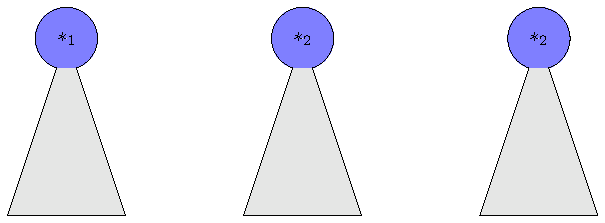
\includegraphics[scale=0.6]{dialoguegame2.pdf}\caption{A Dialogue Game} \end{figure}
into this rooted dialogue game.
\begin{figure}[H]\centering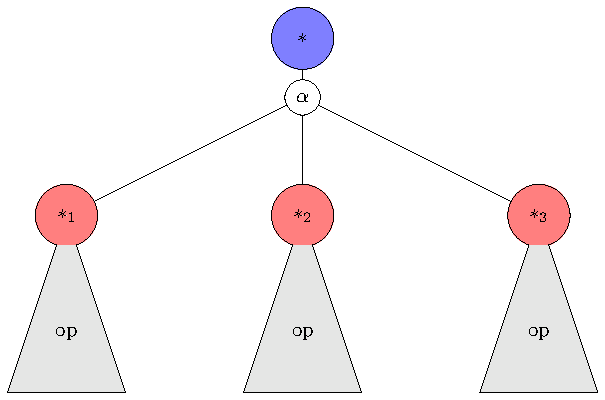
\includegraphics[scale=0.6]{dialoguegame3.pdf} \caption{A Negated Dialogue Game} \end{figure}

Then, we can define the tensor product of a set of negated games ( games of the form $\neg A$) by merging the roots of those games into one root justifying all the cells justified by the original roots.\\
Thus the tensorial product of these negative games : 
\begin{figure}[H]\centering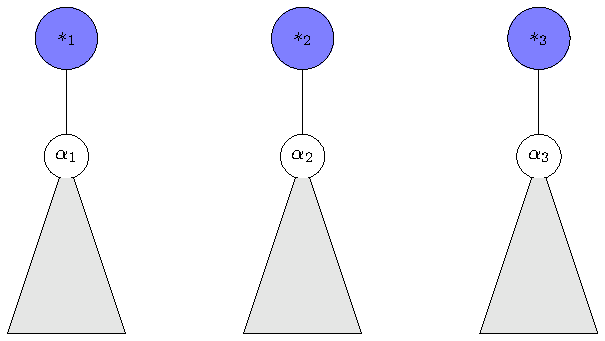
\includegraphics[scale=0.6]{dialoguegame4.pdf} \caption{A sum of Negated Dialogue Games} \end{figure}
is this rooted game :

\begin{figure}[H]\centering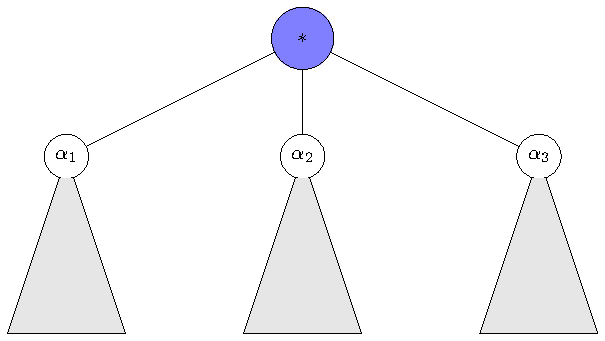
\includegraphics[scale=0.6]{dialoguegame5.pdf} \caption{An example of Tensorial Product} \end{figure}
This is enough to describe all games . Indeed, if you have a non-trivial dialogue game, either it is a set of rooted games ( in which case, the associated formula will be a sum of the games' formulas) or it is a rooted game. \\In this last case, there are two possibilities, either there is only one cell justified by the root (the associated formula is then the negation of a game) or there are several (the associated formula is then a tensor product of negated games).\\ 

We thus have a correspondance as advertised, up to associativity of both connectors and distributivity of the sum over the tensor product.

We will also need one more structure, the game which will contain the arrows from $A$ to $B$ in the category of dialogue games, which will be strategies : The tensorial implication $A \triangleright B := \neg (A \otimes  B^*)$ where $B*$ is the game obtained from $B$ by removing the root and inversing Opponent and Player moves).

\subsection{Sequential Trajectories}

We will look at specific trajectories, that we will call sequential trajectories. Those trajectories are alternating, and all their projections on components are too.( For example, a trajectory on $A \otimes B$ need to be alternating on $A \otimes B$, $A$ and $B$.) Those trajectories will not be able to visit all positions so we need to have a notion of legal positions, they will come in two flavors, positive when one can play an Opponent  move from them and negative when one can play a Player move:
\begin{definition}{Flavored Positions}

 We introduce this notion of flavor by induction over the structure of the games : 
\begin{itemize}
\item The only position of the $1$ game is $+$. 
\item The flavour of positions of a game $A$ are reversed when in the  game $\neg A$
\item  For the tensor product $ A\otimes B$, we have four cases :\\
\begin{itemize}
\item A positive position in $A$ and a positive position in $B$ make a positive position in $A \otimes B$.
\item A negative position in $A$ and a positive position in $B$ make a negative position in $A \otimes B$
\item Similarly, A negative position in $B$ and a positive position in $A$ make a negative position in $A \otimes B$
\item Finally, A negative position in $A$ and a negative position in $B$ make an illegal position in $A \otimes B$. A trajectory getting to such a position would have two Opponent moves more than Player moves, making it impossible to be alternating.\\
\end{itemize}
\end{itemize}
\end{definition}
We can also refine the definition of the underlying graph into a legal underlying graph containing only the legal positions, which will be bipartite ( separated into positive and negative vertices).

\subsection{Reorganizing move orders}

We introduce some equivalence relations over sequential trajectories defined by induction over the structure of the Dialogue games. These definitions are motivated by the wish to understand how  a trajectory can be reorganized into another one when a move is played at a different moment. We also wish to build strategies that would be invariant by those relations to be able to interpret two programs whose only differences are the order of computations in the same way.\\

 We need to have two different equivalence relations because the structure of the dialogue games and of the sequential trajectories highlight major differences between P moves and O moves.
\begin{definition}{Reordering Relations}

Let A be a Dialogue game, x a legal position of A. We define two equivalence relations $\equiv_{OP}$ and $\equiv_ {PO}$ over sequential trajectories reaching $x$ by induction over the structure of $A$ : 
\begin{itemize}
\item for the game $1$, both equivalence relations are the identity.
\item for two trajectories $s$ and $t$ reaching $x$ in a game $\neg A$, we have $s \equiv_{OP} t$ if $s_A \equiv_{PO} t_A$ and $s \equiv_{PO} t$ if $s_A \equiv_{OP} t_A$, where $s_A$ and $t_A$ are the trajectories of $A$ obtained by removing the move associated to the negation.
 
\item for a position x in the tensor product $A \otimes B$, the definitions differ a bit more . Le $s,s',s'',s'''$ be sequences of moves, $O$ and $O_1$ be opponent moves and $P$ and $P_1$ be player moves. 
\begin{itemize}
\item $\equiv_{OP}$ is the equivalence relation generated by the couples: $(s.O.P.O_1.P_1.s' , s.O_1.P_1.O.P.s')$ such that $$s.O.P.O_1.P_1.s'|_A \equiv_{OP} s.O_1.P_1.O.P.s'|_A$$ and $$s.O.P.O_1.P_1.s'|_B \equiv_{OP} s.O_1.P_1.O.P.s'|_B$$ \\

\item $ \equiv_{PO}$ is the equivalence relation generated by the couples $(s.P.s'.O.P_1.s''.O_1.s''', s.P_1.s'.O_1.P.s''.O.s''')$ such that $P,O,P_1,O_1$ all come from the same component,  $$s.P.s'.O.P_1.s''.O_1.s'''|_A \equiv_{PO} s.P_1.s'.O_1.P.s''.O.s'''|_A$$ and $$s.P.s'.O.P_1.s''.O_1.s'''|_B \equiv_{PO} s.P_1.s'.O_1.P.s''.O.s'''|_B$$\\

\end{itemize}
\end{itemize} 
\end{definition}
The definition for the tensor product is a direct consequence of both the structure of the dialogue game and the notion of sequential trajectory. Indeed, it is easy to see that in that case, a P move always follows a O move coming from the same component, and that such a couple of move can be switched with an adjacent couple of moves coming from the other component without causing any upheaval in the trajectory. \\
 \begin{lemma}
Let $A$ be a Dialogue Game, $x$ a legal position, $s=s_0.m.s_1$ a sequential trajectory getting to $x$, $m'$ a move playable at $s_0$ and played in $s$ such that  $m'\neq m$, then there exists $t=s_0.m'.t_1$ a sequential trajectory such that $s\equiv_{OP} t$ or $s\equiv_{PO} t$
\end{lemma}
\begin{proof}
We prove it by induction over the structure of A, the cases of the $1$ game and of the negation being trivial. Let us show it for the tensor product $A_1 \otimes A_2$:\\
There are two cases depending on whether $m$ and $m'$ are $O$ moves or $P$ moves.
\begin{itemize}
\item if they are $O$ moves, we need to consider two sub-cases based on whether $O$ and $O'$ are in the same component of the tensor. 

\begin{itemize}
\item If they are, let us assume $O$ and $O'$ belong to $A_1$.  In this case, we look at the projections over $A_1$. $s|A_1$ is a sequential trajectory reaching $x|_{A_1}$.\\ By induction, we get a sequential trajectory $u_1$ of $A_1$ reaching $x|_{A_1}$ such that $u_1$ starts with $s_0|_{A_1}.O'$. Back in the tensor product, we build $s_1$ in the following way :\\ 
The schedule (how the moves of the different components are ordered) is the same one as $s$. The moves coming from $A_2$ do not change, the moves coming from $s_1$ are in the order of $u_1$. That way, we have $s \equiv_{OP} s_1$, and $s_1$ starts with $s_0.O'$ .\\

\item Otherwise, let us assume $O$ belong to $A_1$ and $O'$ to $A_2$. We have again two subcases depending on whether $O'$ is the first move in $s|_{A_2}$  or not.
\begin{itemize}
\item If it is, we build $s_1$ by moving $O'$ and its answer to the beginning of the trajectory. (it will only switch them with couples of moves of the other component, which is allowed by the definition of $\equiv_{OP})$ .
\item Otherwise, we first do the aforementioned switch to bring the first move  $O''$  of $s\_{A_2}$, and then we apply the method of the first subcase where both O moves are in the same component.
\end{itemize}

\end{itemize}
\item if they are $P$ moves,  they are in the same component, since they are direct answers to the same $O$ move and the trajectories are sequential.\\ Let us assume $P$ and $P'$ belong to $A_1$. In this case, we look at the projections over $A_1$. $s|A_1$ and $t|A_1$ are two trajectories reaching $x|_{A_1}$.\\
 By induction, we get a sequential trajectory $u_1$ of $A_1$ reaching $x|_{A_1}$ such that $u_1$ starts with $s_0|_{A_1}.P'$. Back in the tensor product, we build $s_1$ in the following way :\\
 The schedule (how the moves of the different components are ordered) is the same one as $s$. The moves coming from $A_2$ don't change, the moves coming from $s_1$ are in the order of $u_1$. That way, we have $s \equiv_{PO} s_1$, and $s_1$ starts with $s_0.P'$ . \\


\end{itemize}
\end{proof}



\begin{lemma}
Let A be a Dialogue Game, x a legal position, s and t two sequential trajectories getting to x. Then there is a sequence of trajectories $s_1,...s_n$ such that $s,s_1,... s_n,t$ are a sequence of trajectories related through $\equiv_{OP}$ and $\equiv_{PO}$ alternately and the size of the largest common prefix of $s_i$ and $t$ increases strictly with $i$, (with $s$ being seen as $s_0$. For example,  $s \equiv_{OP} s_1\equiv_{PO} s_2 ... \equiv_{OP} s_n \equiv_{PO} t$
\end{lemma} 
TODO add pictures
\begin{proof}
We prove it by iterating the earlier lemma, first on $s$ and the first move in $t$ that's different from the moves in $s$. It gives us a $s_1$ trajectory as intended. We apply the lemma again on $s_1$ and the first move in $t$ that different from the moves in $s_1$. If the diverging move in the former iteration of the lemma is of the same kind ( Opponent or Playerà as the one in this iteration, we replace $s_1$ by our new result, otherwise we define $s_2$ as our new result. We can continue applying this method, the size of the diverging part of the trajectory decreases strictly with each iteration, so it is a finite process.
\end{proof}

Now that we have introduced our equivalence relations, we will introduce a notion of strategy based on them. We could use equivalence classes of $\equiv_{OP}$  which are deterministic, but they will not have the properties we will need, so we need to add a bit more complexity.


\begin{definition}{Bi-Invariant Strategy}

A strategy $\sigma$ on a dialogue game A is said to be bi-invariant if it only contains sequential trajectories, and : $$\forall s \in \sigma,\forall t, s \equiv_{OP} t \Rightarrow \exists u \in \sigma t \equiv_{PO} u$$
\end{definition}


\subsection{Confluent Strategies}
Let us now look into a new kind of strategies, inspired by rewriting theory. Similarly to the equivalence relations,  the idea comes from the fact that we would want to interpret in the same way two programs that do the same work but handle some computation in a different order (like the two boolean or taking a look at left or right argument first).\\ In terms of trajectories, it means that we want the strategy to be able to play available moves in every possible order. That inspired the definition of confluent strategies : 
\begin{definition}{Confluent Strategy}

A strategy is said to be confluent if it only contains sequential trajectories and if $for s,t \in \sigma$,$m$ a position ,$ s.m \subset t \Rightarrow \exists n, s.m.n \in \sigma \wedge s.m.n \subset t$.\\
It is said to be total if for $s \in \sigma$, $m$ a position, $s.m$ is a valid trajectory $\Rightarrow \exists n, s.m.n \in \sigma$.
\end{definition}
Intuitively, it means that a confluent strategy will explore all paths to a given position in the strategy and that a total strategy will stop exploring the game's tree only when there is no path left.\\

\begin{theorem}

Bi-invariant strategies are exactly the total confluent strategies.
\end{theorem}
\begin{proof}
\begin{itemize}
\item  Let $\sigma$ be a confluent strategy on a dialogue game $A$. Let $s=s_0.O.s_1$ and $t=s_0.O'.t_1$ be two sequential trajectories reaching a legal position$x$, with $s \in \sigma$ and $s \equiv_{OP} t$. By confluency of $\sigma$, there exists $u \in \sigma$ starting with $s_0.O'$ and reaching $x$. There are now three cases depending of the kind of the first divergent move between $t$ and$u$
\begin{itemize}
\item If it is a P move( that we will call $P_t$ and $P_u$, we apply our first lemma to $t$ and $P_u$ to get a sequential trajectory $v$ reaching x, starting with $s_0.O'....P_u$ and such that $t\equiv_{PO} v$. We then choose again between the three cases with $v$ and $u$ instead of $t$ and $u$. 

\item If it is a O move ( that we will call $O_t$ and $O_u$, we apply confluency of $\sigma$ on $u$ and $O_t$ to get a sequential trajectory $w\in \sigma$ reaching $x$ starting with $s_0.O'....O_t$. We then choose again between the three cases with $t$ and $w$ instead of $t$ and $u$.  
\item when there is no more diverging move, we have $t \equiv_{PO} v=u$  with $u\in \sigma$. (we potentially have $t=v$ if there is no divergent move after the initial $\equiv_{OP}$ and confluency applications.  
\end{itemize}
This allows us to build $u$ as needed and thus,$\sigma$ is bi-invariant.
 
\item Let $\sigma$ be a bi-invariant strategy on a dialogue game $A$. Let $s=s_0.O.s_1\in \sigma$ and $O'$ an opponent move playable in $s_0$ and played in $s$. By applying our first lemma to $s$ and $O'$, we get a sequential trajectory $t$ starting with $s_0.O'$ such that $s\equiv_{OP}t$. By bi-invariance of $\sigma$, there exists $u\in \sigma$ such that $t \equiv_{PO} u$. If the $\equiv_{PO}$ causes reorganization of moves before O', u will start like s but diverge on a P move, which breaks determinism, thus u starts with $s_0.O'$ and $\sigma$ is confluent, the answer of $O'$ in $u$ being the needed move.
 

\end{itemize}
\end{proof}

We tried two different methods of describing strategies who act coherently even if the opponent reorders his moves, a local one describing specifically what moves can be reordered and a more global one just stating that the strategy must be able to answer a reordering. What this theorem means is that both the local and global methods are creating the same strategies, ensuring the strength of that definition.  

\begin{theorem}
 Dialogue games and Confluent Strategies form a category.
\end{theorem}
\begin{proof}
We need to check that the usual composition (parallel-hiding) of strategies preserve the properties of confluent strategies.
Let A,B and C be  dialogue games, $\sigma$ a confluent strategy in $A\triangleright B$ and $\tau$ a confluent strategy in $B\triangleright C$. $\sigma \circ \tau$ is a strategy in $A \triangleright C$. We need to check that it is confluent.\\

Let s,t be two trajectories in $\sigma \circ \tau$, $m$ a position, such that $s.m \subset t$. By definition of $\sigma \circ \tau$, there exist $s_\sigma, s_\tau, t_\sigma t_\tau$ trajectories in $\sigma$ and $\tau$ such that $s_\sigma|A=s|A, s_\sigma|B=s_\tau|B, s|C=s_\tau|C$ and $t_\sigma|A=t|A, t_\sigma|B=t_\tau|B, t|C=t_\tau|C$.
We would want to use confluency of $\sigma$ and $\tau$ on $s_\sigma, t_\sigma$ and $s_\tau, t_\tau$ but for that we need to be sure that $s_\sigma \subset t_\sigma$ and $s_\tau \subset t_\tau$.
\begin{figure}[H]\centering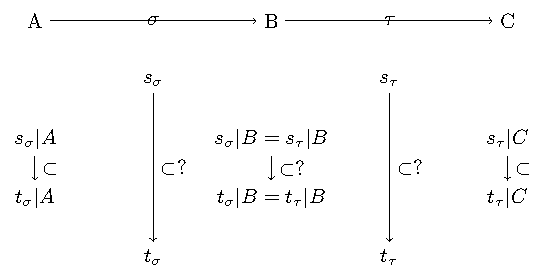
\includegraphics[scale=0.8]{confluency_and_composition_1.pdf}\caption{} \end{figure}

If we play a first move to get to a position $m$ under $t_\tau$, it will be under $s_\tau$ too since it is a move in $C$ and $s_\tau|C \subset t_\tau|C$. we can apply confluency to get a position $n$ such that $m.n$ is both under $s_\tau$ and $t_\tau$ (by determinism of $\tau$).\\ If the move that got us to $n$ is in $C$, we start again by choosing a new move in C under $t_\tau$.\\ If it is in $B$, we can apply the same method on $\sigma$ to get a position $r$ such that n.r is under both $s_\sigma$ and $t_\sigma$ by confluency and determinism. We continue this till we get to $s_\sigma$ and $s_\tau$, ensuring we have  $s_\sigma \subset t_\sigma$ and $s_\tau \subset t_\tau$.\\


We can thus apply confluency on $s_\tau, t_\tau$ and $s_\sigma, t_\sigma$. 
we have two possibilities, the move to get to $m$ from $s$ is a move in $C$ or in $A$.  Let us suppose it is a move in $C$ (We handle the other case similarly).\\ We thus have $s_\tau.m_\tau \subset t_\tau$, where $m_\tau$ is the position we get at when playing the same move than for $m$, but from $s_\tau$. \\By confluency of $\tau$, there exists a move getting us to a position $n_\tau$, such that $s_\tau.m_\tau.n_\tau \in \tau$ and $s_\tau.m_\tau.n_\tau \subset t_\tau$. $n_\tau$ can come from a move in $B$ or in $C$.\\ If it is a move in $C$, we can play the same move from $s.m$ to get the $n$ we need.\\ If it is a move in $B$, it is a move we can play from $s_\sigma$ to get to a position $n_\sigma$ and $s_\sigma.n_\sigma \subset t_\sigma$ since $s_\tau.m_\tau.n_\tau \subset t_\tau$ and $t_\sigma|B=t_\tau|B$. By confluency of $\sigma$, there exists a move getting us to a position $o_\sigma$ such that $s_\sigma.n_\sigma.o_\sigma \subset t_\sigma$ and 
$s_\sigma.n_\sigma.o_\sigma \in \sigma$. Once again, $o_\sigma$ can come from a move in $A$ or in $B$.\\ If it is a move in $A$, we can play the same move from $s.m$ to get the $n$ we need.\\ Otherwise, we repeat the method we have used until we get a move from either A or C. \\It is a finite process as we are staying under $t_\sigma$ and $t_\tau$ each time we add a move.



\end{proof}
\section{Dialogue Games and Graph Games}
In this section, we start by reintroducing Graph Games as described by Hyland and Schalk ~\cite{} , before showing a correspondance between our dialogue games and the graph games, by exhibiting a full and faithful functor from the category of Dialogue games and sequential confluent strategies to the category od graph games and conflict-free strategies.\\


\subsection{Graph Games}
\begin{definition}{Graph Game}

A Graph Game $A$ is given by :
\begin{itemize}
\item A set $A = A_P + A_O$ of positions together with an initial position $*_A$. $A_P$ is the set of Player positiosn ( where Opponent has to move) and $A_O$ the set of Opponent positions.
\item A set of directed edges that makes the graph bipartite and  acyclic.
\item a play in the game is a sequence of positions $*_A=a_0.a_1...a_n$ such that for all $i$ $a_i \rightarrow a_{i+1}$
\end{itemize}
\end{definition}

\begin{definition}{Reachable Positions}

Let $\alpha$ be a partial function from $A_O$ to $A_P$ such that $a\rightarrow \alpha(a)$ when it is defined. The set of reachable positions for $\alpha$ $R(\alpha)$ is defined by induction in the following way : 
\begin{itemize}
\item $*_A \in R(\alpha)$
\item if $a \in R(\alpha)\bigcap A_P$ and $a\rightarrow a'$ then $a'\in R(\alpha)$. 
\item if $a \in R(\alpha)\bigcap A_O$, $\alpha(a)$ is defined (and thus $a\rightarrow \alpha(a)) $ then $\alpha(a)\in R(\alpha)$.
\end{itemize}
 
We then define a pre-strategy as a partial function $\alpha$ from $A_O$ to $A_P$ such that $a\rightarrow \alpha(a)$ when it is defined and that its domain of definition is a subset of $R(\alpha)$.
\end{definition}

\begin{definition}{Strategy}

a strategy of the game $A$ is a conflict-free pre-strategy, that is a pre-strategy such that if $a \in R(\alpha)\bigcap A_P$ is reachable from $a' \in R(\alpha)\bigcap A_O$ then $\alpha (a')$ is defined and a is reachable from $\alpha(a')$. 
\end{definition}

\begin{definition}{Multiplicative Structure}
\begin{itemize}
\item The tensor $A\otimes B$ of two graph games $A$ and $B$ is the graph game whose player positions are in $A_P \times B_P$ and whose Opponent positions are in $(A_P \times B_O) + (A_O \times B_P)$. Its initial position is $ (*_A, *_B)$ and there is a move from $(a,b)$ to $(a',b')$ when either there is a move from $a$ to $a'$ in A and $b=b'$ or there is a move from $b$ to $b'$ in B and $a=a'$.\\
\item The linear function space $A \multimap B$ of two graph games $A$ and $B$ is the graph game whose player positions are in $(A_P \times B_P) + (A_O \times B_O)$ and whose opponent positions are in $A_P \times B_O$. Its initial position is $ (*_A, *_B)$ and there is a move from $(a,b)$ to $(a',b')$ when either there is a move from $a$ to $a'$ in A and $b=b'$ or there is a move from $b$ to $b'$ in B and $a=a'$.\\
\end{itemize}
\end{definition}

We can then define the category of Graph Games and Conflict-free Strategies as the category whose objects are the graph games and whose arrows from $A$ to $B$ are the conflict-free strategies of the game $A\multimap B$. The composition of strategies is defined by a process based on parallel composition plus hiding of trajectories in the graph.
  
\subsection{Proving the correspondance}
\begin{theorem}
There exists a full and faithful functor $F$ between the category of dialogue games and sequential confluent strategies, and the category of graph games and conflict-free strategies.
\end{theorem} 

\begin{proof}
Let us start by defining this functor :
\begin{itemize}
\item Let A be a dialogue game. we define $F(A)$ as the game played on the underlying legal graph of $A$ with the positive positions being the Player vertices and the negative positions being the Opponent vertices. \\Given the structural definitions of both graph games and legal positions of dialogue games, one can easily note that the functor respects the structure of the game . $F(1_{D})=1_{G}, F(A \otimes B) = F(A) \otimes F(B), F(\neg A) = \neg F(A)$\\

\item  Let $\sigma$ be a sequential and confluent strategy on a dialogue game $A$. We define the conflict-free strategy $F(\sigma)$ on the graph game $F(A)$ in the following way:\\ 
Let s be a non-void trajectory in $\sigma$, then $s=s_0.m.n$, with $s_0$ a trajectory, $m$ an Opponent move, and $n$ a Player move. $\{ s_0,m\}$ is thus an negative position, thus an Opponent vertex in $F(A)$. Similarly, $\{s_0,m,n\}$ is a Player vertex in $F(A)$.\\ We define $F(\sigma)(\{ s_0,m\}) = \{s_0,m,n\}$ and do so for each trajectory in $\sigma$. This gives us a partial function as intended ( thanks to the determinism of $\sigma$), which is also conflict-free thanks to the confluency of $\sigma$.\\
 Indeed,  le t$a$ be a player position in $R(F(\sigma))$ and $a'$ an opponent position in $R(F(\sigma))$ such that $a$ is reachable from $a'$.\\ The inductive construction of $R(F(\sigma))$ can easily be seen as an inductive way to build trajectories in the game $A$ following $\sigma$.\\
 Thus $a\in R(F(\sigma))$  translates into "there is a trajectory in $\sigma$ reaching $a$ if $a$ is a Player position. Otherwise, it translates into "there is a trajectory $t$ in $\sigma$ and an opponent move $O$ such that t.O reaches $a$' .\\
Thus we get a trajectory s in $\sigma$  reaching $s$ and another one $t=t_0.O$ such that $t_0$ is in $\sigma$,  reaching $a'$. Since $a$ is reachable from $a$, it means that $t \subset s$. by confluency of $\sigma$ , there exists  a Player move $P$ such that $t.P\subset s$ and $t.P$ is in $\sigma$ and $t.P$ can be completed to reach $a$.\\ 
Applying our translation to those statements gives us $F(\sigma) (a)$ is defined (and equal to $\{t.P\}$) and a' is reachable from $F(\sigma) (a)$ \\

One can note that we have been able to do the translation for strategies of all dialogue games, and not only for the ones that are arrows in our category.\\

\end{itemize}
let us now check the remaining properties of the functor : 

\begin{itemize}
\item The aforementioned construction of $F$ makes it easy to prove that the image of the copycat strategy of a dialogue game $A\rhd A$ is the copycat strategy of the graph game $F(A)\rightarrow F(A)$, the answer to an Opponent move played in one component always being the same move played in the other component.\\

\item Let $A, B, C$ be three dialogue games, $\sigma$ a strategy $ A \rhd B$ and $\tau$ a strategy in $B \rhd C$. We have $F(\sigma o \tau)( a,c) = (a', c')$ when there is a trajectory in $\sigma o \tau$ moving from $(a,c)$ to $(a',c')$ , which, by parallel composition plus hiding, means that there is a trajectory in $\sigma$ moving from $a,b$ to $a',b'$ and a trajectory in $\tau$ moving from $b,c$ to $b',c'$ composing correctly. Those trajectories are the same in the graph games, meaning that they belong in $F(\sigma)$ and $F(\tau)$, and thus the initial trajectory belongs to $F(\sigma) o F(\tau)$. \\

\end{itemize}
Furthermore, the functor is indeed fully faithful.\\
 One only has to build the set of trajectories $G(\alpha)$ back from the partial function $\alpha$ to get the strategy that produced it, by using the inductive construction of the reachable set fo the strategy.\\
 The set of built trajectories is a strategy since the partial function gives at most one answer to a given Opponent vertex, which means at most one playable P  move when waiting for one in a trajectory. The confluency comes from the fact that the function is conflict-free. \\Let $s$ and $t$ two trajectories of the dialogue game belonging to $G(\alpha)$  with $s \subset t$ and a move $O$ playable from $s$ and played in $t$. From the construction of the reachable set, we get that $\{t\} \in R(\alpha)$ is reachable from $\{s,O\} \in R(\alpha)$. since $\alpha$ is conflict-free,  $\alpha(\{s,O\}$ is defined and can reach $t$. \\Thus we have a player move P to play after $s.O$ and  $s.O.P \subset t$. $G(\alpha)$ is confluent. Furthermore, by construction, we have $G=F^{-1}$  \\



Thus we have built a bijection between the confluent strategies of a given dialogue game and the conflict-free strategies of the associated graph game, making the functor fully faithful.


\end{proof}



\section*{Conclusion}


\bibliography{biblio}
\bibliographystyle{splncs03}

\clearpage

\section*{Appendix}
\end{document}

